
%% bare_conf.tex 
%% V1.2
%% 2002/11/18
%% by Michael Shell
%% mshell@ece.gatech.edu
%% 
%% NOTE: This text file uses UNIX line feed conventions. When (human)
%% reading this file on other platforms, you may have to use a text
%% editor that can handle lines terminated by the UNIX line feed
%% character (0x0A).
%% 
%% This is a skeleton file demonstrating the use of IEEEtran.cls 
%% (requires IEEEtran.cls version 1.6b or later) with an IEEE conference paper.
%% 
%% Support sites:
%% http://www.ieee.org
%% and/or
%% http://www.ctan.org/tex-archive/macros/latex/contrib/supported/IEEEtran/ 
%%
%% This code is offered as-is - no warranty - user assumes all risk.
%% Free to use, distribute and modify.

% *** Authors should verify (and, if needed, correct) their LaTeX system  ***
% *** with the testflow diagnostic prior to trusting their LaTeX platform ***
% *** with production work. IEEE's font choices can trigger bugs that do  ***
% *** not appear when using other class files.                            ***
% Testflow can be obtained at:
% http://www.ctan.org/tex-archive/macros/latex/contrib/supported/IEEEtran/testflow


% Note that the a4paper option is mainly intended so that authors in
% countries using A4 can easily print to A4 and see how their papers will
% look in print. Authors are encouraged to use U.S. letter paper when 
% submitting to IEEE. Use the testflow package mentioned above to verify
% correct handling of both paper sizes by the author's LaTeX system.
%
% Also note that the "draftcls" or "draftclsnofoot", not "draft", option
% should be used if it is desired that the figures are to be displayed in
% draft mode.
%
% This paper can be formatted using the peerreviewca
% (instead of conference) mode.
\documentclass[conference]{IEEEtran}
% If the IEEEtran.cls has not been installed into the LaTeX system files, 
% manually specify the path to it:
% \documentclass[conference]{../sty/IEEEtran} 


% some very useful LaTeX packages include:

%\usepackage{cite}      % Written by Donald Arseneau
                        % V1.6 and later of IEEEtran pre-defines the format
                        % of the cite.sty package \cite{} output to follow
                        % that of IEEE. Loading the cite package will
                        % result in citation numbers being automatically
                        % sorted and properly "ranged". i.e.,
                        % [1], [9], [2], [7], [5], [6]
                        % (without using cite.sty)
                        % will become:
                        % [1], [2], [5]--[7], [9] (using cite.sty)
                        % cite.sty's \cite will automatically add leading
                        % space, if needed. Use cite.sty's noadjust option
                        % (cite.sty V3.8 and later) if you want to turn this
                        % off. cite.sty is already installed on most LaTeX
                        % systems. The latest version can be obtained at:
                        % http://www.ctan.org/tex-archive/macros/latex/contrib/supported/cite/

\usepackage{graphicx}  % Written by David Carlisle and Sebastian Rahtz
                        % Required if you want graphics, photos, etc.
                        % graphicx.sty is already installed on most LaTeX
                        % systems. The latest version and documentation can
                        % be obtained at:
                        % http://www.ctan.org/tex-archive/macros/latex/required/graphics/
                        % Another good source of documentation is "Using
                        % Imported Graphics in LaTeX2e" by Keith Reckdahl
                        % which can be found as esplatex.ps and epslatex.pdf
                        % at: http://www.ctan.org/tex-archive/info/
% NOTE: for dual use with latex and pdflatex, instead load graphicx like:
%\ifx\pdfoutput\undefined
%\usepackage{graphicx}
%\else
%\usepackage[pdftex]{graphicx}
%\fi

% However, be warned that pdflatex will require graphics to be in PDF
% (not EPS) format and will preclude the use of PostScript based LaTeX
% packages such as psfrag.sty and pstricks.sty. IEEE conferences typically
% allow PDF graphics (and hence pdfLaTeX). However, IEEE journals do not
% (yet) allow image formats other than EPS or TIFF. Therefore, authors of
% journal papers should use traditional LaTeX with EPS graphics.
%
% The path(s) to the graphics files can also be declared: e.g.,
% \graphicspath{{../eps/}{../ps/}}
% if the graphics files are not located in the same directory as the
% .tex file. This can be done in each branch of the conditional above
% (after graphicx is loaded) to handle the EPS and PDF cases separately.
% In this way, full path information will not have to be specified in
% each \includegraphics command.
%
% Note that, when switching from latex to pdflatex and vice-versa, the new
% compiler will have to be run twice to clear some warnings.


%\usepackage{psfrag}    % Written by Craig Barratt, Michael C. Grant,
                        % and David Carlisle
                        % This package allows you to substitute LaTeX
                        % commands for text in imported EPS graphic files.
                        % In this way, LaTeX symbols can be placed into
                        % graphics that have been generated by other
                        % applications. You must use latex->dvips->ps2pdf
                        % workflow (not direct pdf output from pdflatex) if
                        % you wish to use this capability because it works
                        % via some PostScript tricks. Alternatively, the
                        % graphics could be processed as separate files via
                        % psfrag and dvips, then converted to PDF for
                        % inclusion in the main file which uses pdflatex.
                        % Docs are in "The PSfrag System" by Michael C. Grant
                        % and David Carlisle. There is also some information 
                        % about using psfrag in "Using Imported Graphics in
                        % LaTeX2e" by Keith Reckdahl which documents the
                        % graphicx package (see above). The psfrag package
                        % and documentation can be obtained at:
                        % http://www.ctan.org/tex-archive/macros/latex/contrib/supported/psfrag/

%\usepackage{subfigure} % Written by Steven Douglas Cochran
                        % This package makes it easy to put subfigures
                        % in your figures. i.e., "figure 1a and 1b"
                        % Docs are in "Using Imported Graphics in LaTeX2e"
                        % by Keith Reckdahl which also documents the graphicx
                        % package (see above). subfigure.sty is already
                        % installed on most LaTeX systems. The latest version
                        % and documentation can be obtained at:
                        % http://www.ctan.org/tex-archive/macros/latex/contrib/supported/subfigure/

%\usepackage{url}       % Written by Donald Arseneau
                        % Provides better support for handling and breaking
                        % URLs. url.sty is already installed on most LaTeX
                        % systems. The latest version can be obtained at:
                        % http://www.ctan.org/tex-archive/macros/latex/contrib/other/misc/
                        % Read the url.sty source comments for usage information.

%\usepackage{stfloats}  % Written by Sigitas Tolusis
                        % Gives LaTeX2e the ability to do double column
                        % floats at the bottom of the page as well as the top.
                        % (e.g., "\begin{figure*}[!b]" is not normally
                        % possible in LaTeX2e). This is an invasive package
                        % which rewrites many portions of the LaTeX2e output
                        % routines. It may not work with other packages that
                        % modify the LaTeX2e output routine and/or with other
                        % versions of LaTeX. The latest version and
                        % documentation can be obtained at:
                        % http://www.ctan.org/tex-archive/macros/latex/contrib/supported/sttools/
                        % Documentation is contained in the stfloats.sty
                        % comments as well as in the presfull.pdf file.
                        % Do not use the stfloats baselinefloat ability as
                        % IEEE does not allow \baselineskip to stretch.
                        % Authors submitting work to the IEEE should note
                        % that IEEE rarely uses double column equations and
                        % that authors should try to avoid such use.
                        % Do not be tempted to use the cuted.sty or
                        % midfloat.sty package (by the same author) as IEEE
                        % does not format its papers in such ways.

%\usepackage{amsmath}   % From the American Mathematical Society
                        % A popular package that provides many helpful commands
                        % for dealing with mathematics. Note that the AMSmath
                        % package sets \interdisplaylinepenalty to 10000 thus
                        % preventing page breaks from occurring within multiline
                        % equations. Use:
%\interdisplaylinepenalty=2500
                        % after loading amsmath to restore such page breaks
                        % as IEEEtran.cls normally does. amsmath.sty is already
                        % installed on most LaTeX systems. The latest version
                        % and documentation can be obtained at:
                        % http://www.ctan.org/tex-archive/macros/latex/required/amslatex/math/



% Other popular packages for formatting tables and equations include:

%\usepackage{array}
% Frank Mittelbach's and David Carlisle's array.sty which improves the
% LaTeX2e array and tabular environments to provide better appearances and
% additional user controls. array.sty is already installed on most systems.
% The latest version and documentation can be obtained at:
% http://www.ctan.org/tex-archive/macros/latex/required/tools/

% Mark Wooding's extremely powerful MDW tools, especially mdwmath.sty and
% mdwtab.sty which are used to format equations and tables, respectively.
% The MDWtools set is already installed on most LaTeX systems. The lastest
% version and documentation is available at:
% http://www.ctan.org/tex-archive/macros/latex/contrib/supported/mdwtools/


% V1.6 of IEEEtran contains the IEEEeqnarray family of commands that can
% be used to generate multiline equations as well as matrices, tables, etc.


% Also of notable interest:

% Scott Pakin's eqparbox package for creating (automatically sized) equal
% width boxes. Available:
% http://www.ctan.org/tex-archive/macros/latex/contrib/supported/eqparbox/



% Notes on hyperref:
% IEEEtran.cls attempts to be compliant with the hyperref package, written
% by Heiko Oberdiek and Sebastian Rahtz, which provides hyperlinks within
% a document as well as an index for PDF files (produced via pdflatex).
% However, it is a tad difficult to properly interface LaTeX classes and
% packages with this (necessarily) complex and invasive package. It is
% recommended that hyperref not be used for work that is to be submitted
% to the IEEE. Users who wish to use hyperref *must* ensure that their
% hyperref version is 6.72u or later *and* IEEEtran.cls is version 1.6b 
% or later. The latest version of hyperref can be obtained at:
%
% http://www.ctan.org/tex-archive/macros/latex/contrib/supported/hyperref/
%
% Also, be aware that cite.sty (as of version 3.9, 11/2001) and hyperref.sty
% (as of version 6.72t, 2002/07/25) do not work optimally together.
% To mediate the differences between these two packages, IEEEtran.cls, as
% of v1.6b, predefines a command that fools hyperref into thinking that
% the natbib package is being used - causing it not to modify the existing
% citation commands, and allowing cite.sty to operate as normal. However,
% as a result, citation numbers will not be hyperlinked. Another side effect
% of this approach is that the natbib.sty package will not properly load
% under IEEEtran.cls. However, current versions of natbib are not capable
% of compressing and sorting citation numbers in IEEE's style - so this
% should not be an issue. If, for some strange reason, the user wants to
% load natbib.sty under IEEEtran.cls, the following code must be placed
% before natbib.sty can be loaded:
%
% \makeatletter
% \let\NAT@parse\undefined
% \makeatother
%
% Hyperref should be loaded differently depending on whether pdflatex
% or traditional latex is being used:
%
%\ifx\pdfoutput\undefined
%\usepackage[hypertex]{hyperref}
%\else
%\usepackage[pdftex,hypertexnames=false]{hyperref}
%\fi
%
% Pdflatex produces superior hyperref results and is the recommended
% compiler for such use.

\usepackage{epstopdf}


% *** Do not adjust lengths that control margins, column widths, etc. ***
% *** Do not use packages that alter fonts (such as pslatex).         ***
% There should be no need to do such things with IEEEtran.cls V1.6 and later.



\begin{document}

% paper title
\title{Robust Control of a Radio Controlled Car Driving on Two Wheels }

% author names and affiliations
% use a multiple column layout for up to three different
% affiliations

\author{\authorblockN{Daniel Robert Meier}
\authorblockA{danielme@student.ethz.ch\\
D-MAVT, ETH Zurich}
}

\maketitle

\begin{abstract}

This paper presents the modelling and control of an RC-car driving on two wheels. In order to deal with a variety of uncertainties, a robust control approach is chosen. Therefore, perturbations are modelled in order to deal with actuator uncertainties as well as different geometries. The controller design with D-K iteration is compared to the design with a $H_{\infty}$ controller.

\end{abstract}

\section{Introduction}

This project presents a robust control approach in order to stabilize a radio controlled car on two wheels. Figure \ref{figure:arab_driving}\footnote{Picture source: http://list25.com/} shows this driving mode with a real car. A car on two wheels is an unstable and nonlinear system and therefore needs to be actively controlled. Due to several sources of uncertainty (such as geometry or an imprecise steering) a robust controller is desirable.

\begin{figure}[h]
\centering
  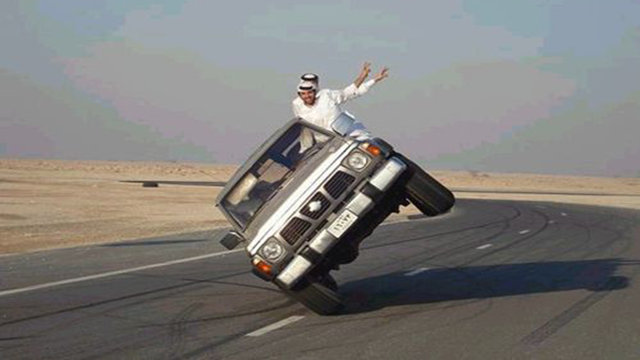
\includegraphics[width=.47\textwidth]{pics/drivesensibly.png} 
  \caption{Two-wheeled driving in a real car}  
  \label{figure:arab_driving}
\end{figure}

The R/C car which will be modelled is a HPI Sprint, as depicted in Figure \ref{figure:hpi_sprint}\footnote{Picture source: http://www.rcnitrotalk.com}. Its length is about 430mm with a weight of about 1.2kg. It can be controlled with the front wheels, which have an angle $\alpha$, resulting in a turning rate $\Psi$. The car is actuated with a DC motor on the rear wheels and drives with the velocity $v$, which is assumed to be constant.  

\begin{figure}[h!]
\centering
  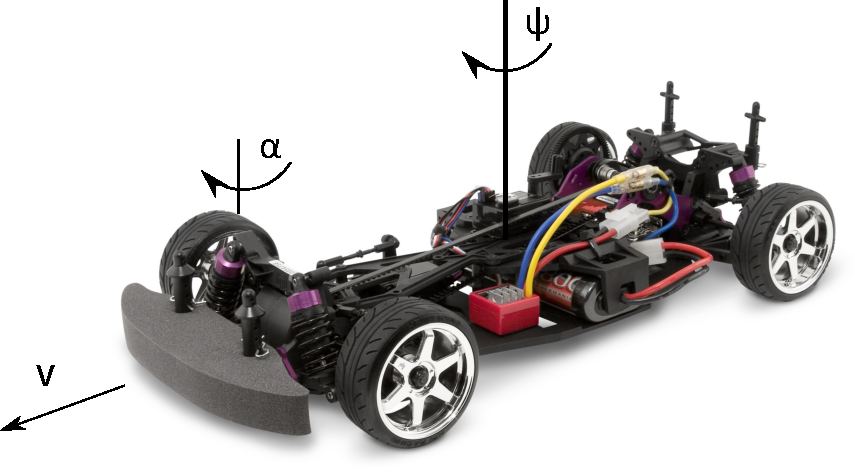
\includegraphics[width=.3\textwidth]{pics/hpisprintgeom.pdf} 
  \caption{HPI Sprint}  
  \label{figure:hpi_sprint}
\end{figure}

The controller has in- \& outputs as depicted in Table \ref{figure:controlinout}. The angle command $\alpha$ is sent to the servo which actuated the steering. As a input the roll angle $\rho$ is chosen since it also corresponds to the vehicles direction. A design with a position input would be interesting for simulation purposes, however not suitable since the real system does not comprise sensors to observe it.

\begin{table}[h]
\begin{center}
\begin{tabular}{|l||l|l|}
\hline
 		& Input 		& Output\\
\hline
SISO 	& Roll angle $\rho$ 	& Steering angle $\alpha$\\
\hline
\end{tabular}
\caption{In- and outputs of the control system}  
\label{figure:controlinout}
\end{center}
\end{table}


\section{Prior Work}

Arndt \cite{bib:arndt} presented an approach to control a car on two wheels, however not using an optimal controller. Moreover, their car has significantly bigger tires, more inertia and a higher center of gravity which facilitates control. Liu \cite{bib:liu} developed a PID approach to control a car driving on two wheels.

\section{Dynamic System Model}

The system model consists of the steering mechanism, the roll angle dependant mapping of the steering angle and the vehicle body dynamics. It is set up as depicted in Figure \ref{figure:P_car}. 

\begin{figure}[h]
\centering
  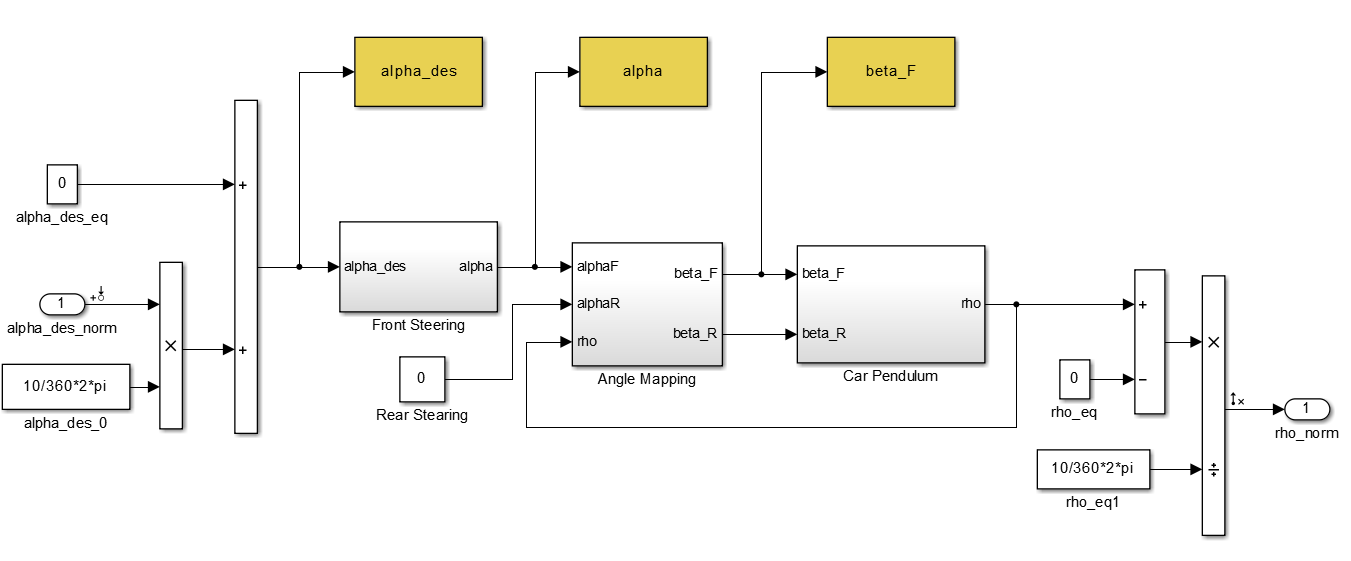
\includegraphics[width=.47\textwidth]{pics/P_car.png} 
  \caption{Normalized plant}  
  \label{figure:P_car}
\end{figure}

The angle $\rho$ depicts the cars attitude as introduced in Figure \ref{figure:car_from_back}\footnote{Source of car picture: http://www.4vector.com}. Accordingly, there is one equilibrium point ($\dot{\Psi} = \dot{\rho} = \dot{\alpha} = 0$) which is dependant on the weight distribution of the car and its center of gravity (COG). This equilibrium point is also chosen at the operating point. As normalization factors, a steering angle $\alpha_{0}=10°$ and a roll angle $\rho_{0}=10°$ is chosen.

\begin{figure}[h]
\centering
  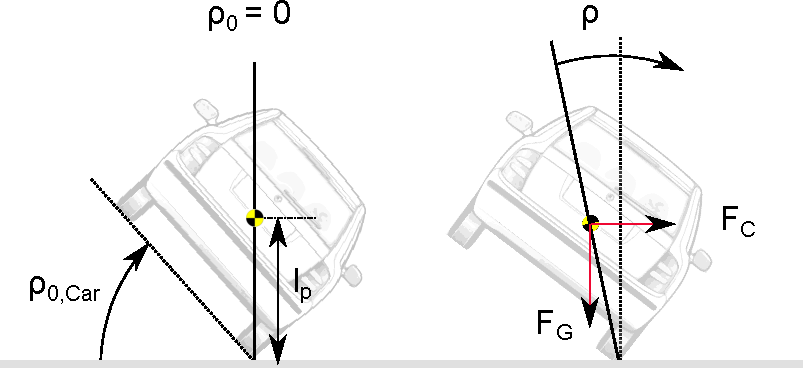
\includegraphics[width=.47\textwidth]{pics/car_from_back} 
  \caption{Convention of roll angle: The state $\rho$ depicts the angle around the equilibrium point (where the car's GOG is right above the line of the two wheels). $\rho_{0,car}$ is a geometrical constant which describes the cars attitude at the equilibrium.}  
  \label{figure:car_from_back}
\end{figure}



\subsection{Modelling Assumptions}

\begin{itemize}
    \item Constant velocity $v$. The dynamics of motor are slower than the dynamics of the steering and the balancing.
    \item Coriolis force is neglected, since it is small for small steering angles.
    \item Contact model: Tires have infinite grip and follow exactly the steering direction.
\end{itemize}


\subsection{Steering}

The front wheel steering is modelled as a second order system as described by equation \ref{eq:steering}. $\alpha _{desired}$ is the systems control input, $\omega$ and $\zeta$ are chosen to match the dynamics as realistic as possible.

\begin{equation}
\frac{{{d^2}}}{{d{t^2}}}\alpha  =  - 2\zeta \omega \dot \alpha  - {\omega ^2}\left( {\alpha  - {\alpha _{desired}}} \right)
\label{eq:steering}
\end{equation}

To get the effective steering angle $\beta$, a nonlinear mapping is required. It is depicted by Figure \ref{figure:angle_plot} and implemented in the block \textit{Angle Mapping}. It can be seen that steering inputs lead to high effective angles when operating at a high roll angle. Moreover the nonlinearity is more significant at higher roll angles $\rho$.

\begin{figure}[Hhh]
\centering
  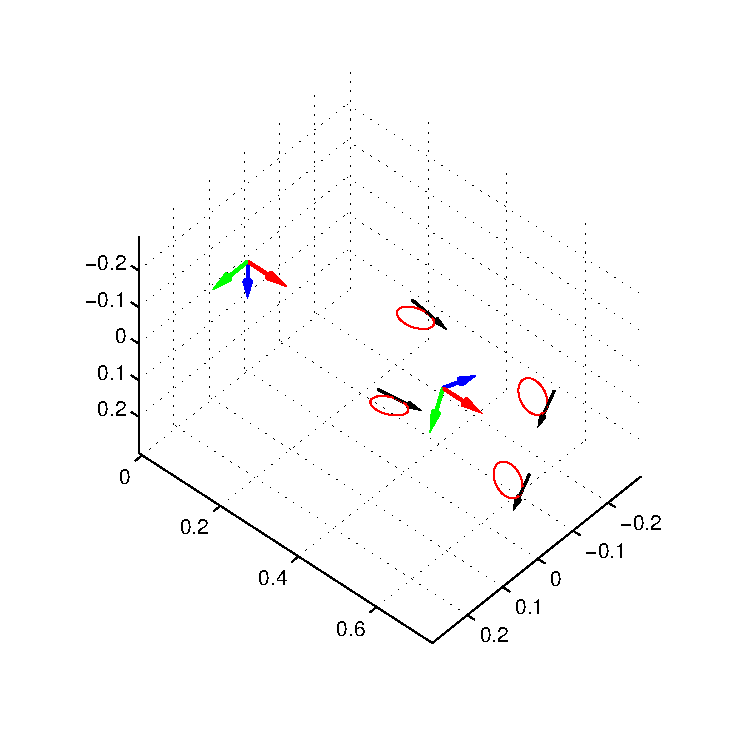
\includegraphics[width=.3\textwidth]{pics/car_roll.eps} 
  \caption{Car with a non-zero roll angle. The effective steering angle $\beta$ is different to the steering angle $\alpha$}  
  \label{figure:car_roll}
\end{figure}

\begin{figure}[Hhh]
\centering
  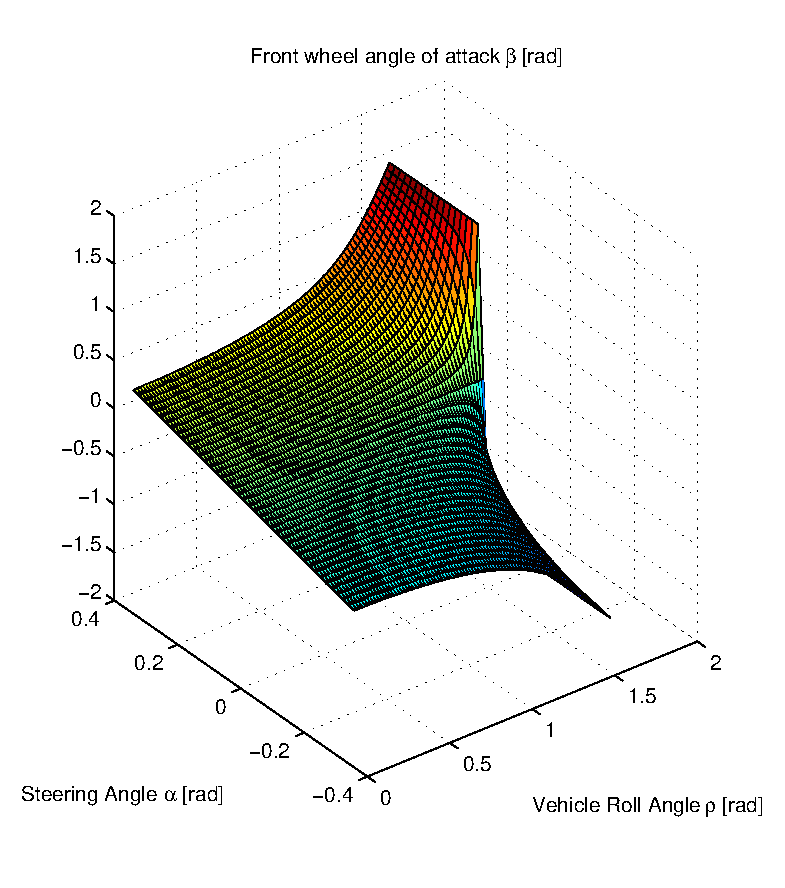
\includegraphics[width=.4\textwidth]{pics/angle_plot.eps} 
  \caption{Angle mapping: Steering angle $\alpha$ vs. effective steering angle $\beta$}  
  \label{figure:angle_plot}
\end{figure}


\subsection{Body dynamics}

The vehicle is modelled as depicted in Figure \ref{figure:geometry}. The gravitational force $F_G$ and the centripetal force $F_C$ are defined as:

\begin{equation}
{F_G} = m \cdot g
\end{equation}

\begin{equation}
{F_C} = \cos \left( {{\gamma _c}} \right) \cdot m \cdot {{\dot \psi }^2} \cdot {l_{ZM}}
\end{equation}

\begin{figure}[h]
\centering
  \includegraphics[width=.47\textwidth]{pics/setup} 
  \caption{Geometry in a turning position}  
  \label{figure:geometry}
\end{figure}

$m$ is the vehicles mass, $l_{ZM}$ the distance between the center of rotation and the GOG and $\dot \psi$ the turning rate of the car. The factor $\cos \left( {{\gamma _c}} \right)$ takes into account that the centripetal force is not necessarily perpendicular to the roll axis of rotation of the car. This factor however can be neglected since it has only very small deviations from $1$. With $\dot \psi  = \frac{v}{{{l_{ZR}}}}$ and ${l_{ZM}} \approx {l_{ZR}}$, the centripetal force can therefore be expressed as:

\begin{equation}
{F_C} \approx m \cdot \frac{{{v^2}}}{{{l_w}}} \cdot \frac{{\sin \left( {{\beta _F} - {\beta _R}} \right)}}{{\cos \left( {{\beta _F}} \right)}}
\end{equation}

$v$ is the vehicles velocity, $l_w$ the distance between the two wheels, $\beta_F$ and $\beta_R$ the front and rear effective steering angles resulting from the non-linear mapping. The resulting differential equation is given as:


\begin{equation}
\frac{{d\rho }}{{dt}} = \dot \rho
\end{equation}

\begin{equation}
\frac{{d\dot \rho }}{{dt}} = \frac{1}{{m \cdot {l_p}}}\left( {\sin \rho  \cdot {F_G} - \cos \rho  \cdot {F_C}} \right)
\end{equation}


\subsection{States}

As a result, the plant consists of the states shown in Table \ref{figure:states}.

\begin{table}[h]
\begin{center}
\begin{tabular}{|l||l|l|l|}
\hline
Variable 		& Description 		& Unit		& Operating point \\
\hline
$\alpha$ 		& Steering angle 	& $rad$	& 0\\
\hline
$\dot \alpha$	& Steering rate 	& $rad/s$	& 0\\
\hline
$\rho$			& Roll angle 		& $rad$	& 0\\
\hline
$\dot \rho$		& Roll rate 		& $rad/s$	& 0\\
\hline
\end{tabular}
\caption{States of the nominal plant}  
\label{figure:states}
\end{center}
\end{table}


\section{Uncertainty Modelling}


%For the introduced control problen, the following sources for uncertainty comprise are considered:
%
%\begin{itemize}
%    \item Geometry: Inertia tensor and mass. The weight distribution for instance determines the equilibrium point $\bar{\beta}$
%    \item Steering: The effect of the steering angle is dependent on the vehicles tilt angle $\beta$ and nonlinear. Uncertainties can cause significant error
%    \item Contact model for wheel - ground interaction
%    \item Engine behaviour
%    \item External disturbances such as wind
%\end{itemize}

In order to deal with uncertainties, perturbations were introduced to the model. The uncertainty of the angle is modelled as a constant with value $0.1$, which is equivalent to 1 degree. Also, the actuator has a uncertainty of $0.05$ (0.5 degree).

\begin{equation}
\label{eg:W_rho}
{W_{rho}} = 0.1
\end{equation}

\begin{equation}
{W_{alpha}} = 0.05
\end{equation}

Performance weights are chosen as in equation \ref{eg:W_rhop} and \ref{eg:W_alphap}. In order to avoid high frequency actuation commands, $W_{alpha,performance}$ is chosen to act as a high frequency penalty.

\begin{equation}
\label{eg:W_rhop}
{W_{rho,performace}} = \frac{{10}}{{10 \cdot s + 1}}
\end{equation}

\begin{equation}
\label{eg:W_alphap}
{W_{alpha,performance}} = \frac{{0.04 \cdot \left( {1 + 0.4 \cdot s} \right)}}{{100 + 0.1 \cdot s}}
\end{equation}

Noise is assumed to be constant over the whole spectrum. Disturbances should be rejected in low frequencies.

\begin{equation}
{W_{rho,noise}} = 0.025
\end{equation}

\begin{equation}
{W_{rho,disturbance}} = \frac{{2.5}}{{5 \cdot s + 1}}
\end{equation}

Figure \ref{figure:weights} shows these weights graphically.

\begin{figure}[h]
\centering
  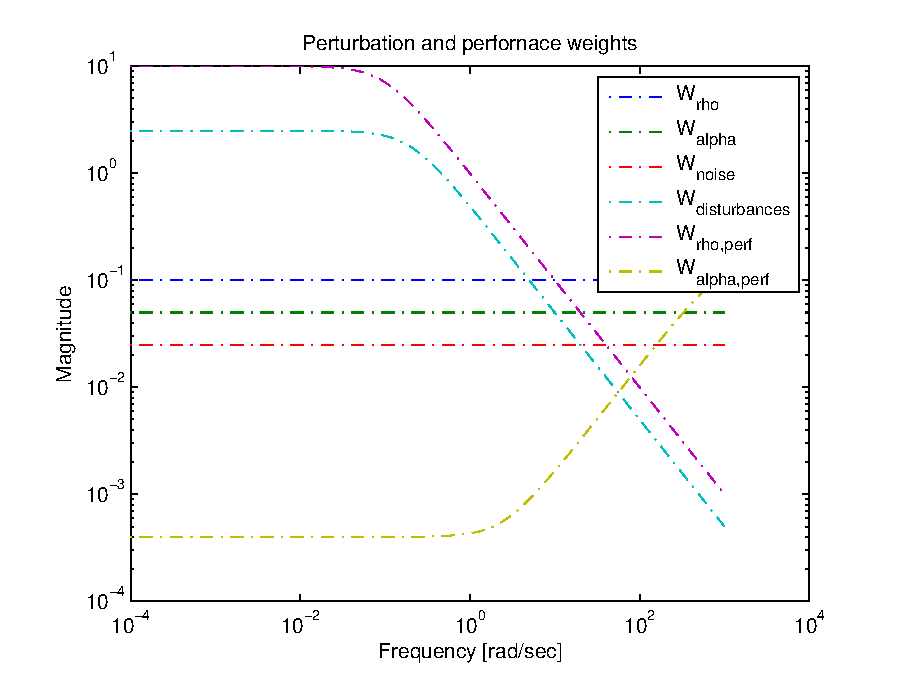
\includegraphics[width=.47\textwidth]{pics/weights.eps} 
  \caption{Weights of the weighted plant}  
  \label{figure:weights}
\end{figure}

As a result, the weighted plant looks as depicted in \ref{figure:model_car}. The inputs are described in Table \ref{figure:model_car_inputs} and the outputs in Table \ref{figure:model_car_outputs}.

\begin{figure}[h]
\centering
  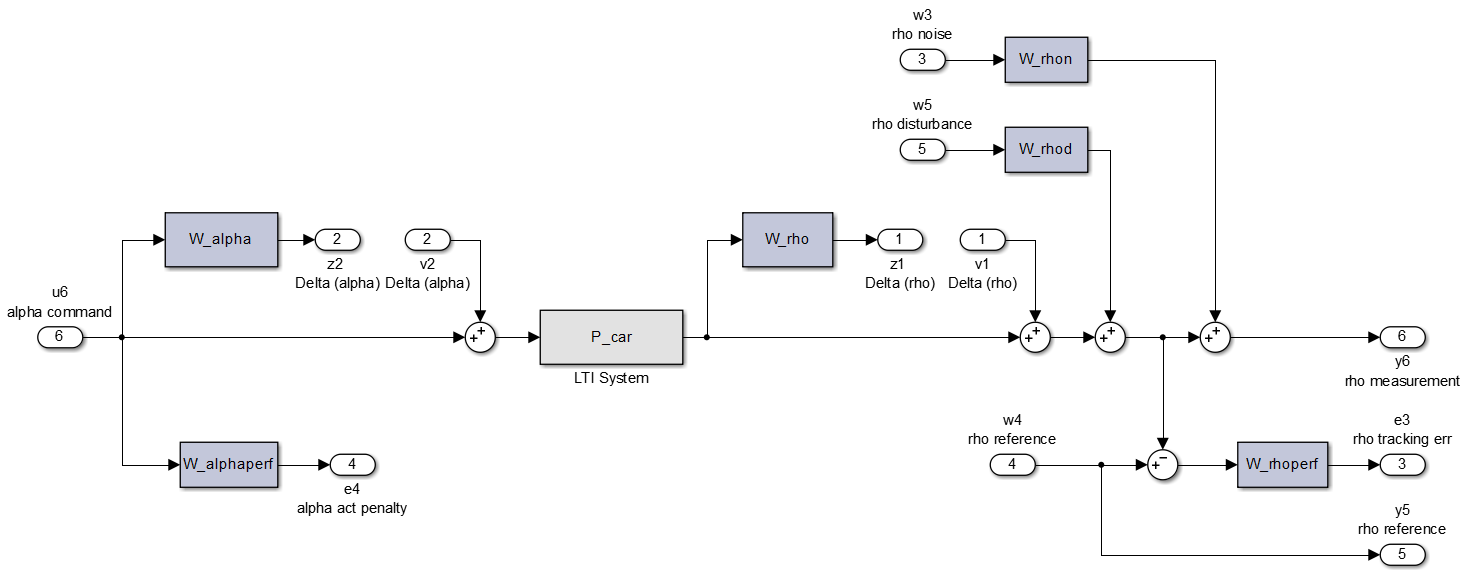
\includegraphics[width=.47\textwidth]{pics/model_car.png} 
  \caption{Weighted plant}  
  \label{figure:model_car}
\end{figure}


\begin{table}[h]
\begin{center}
\begin{tabular}{|l||l|}
\hline
Vector 		& Description 		\\
\hline
$v1$ 		& Delta ($\rho$) 	\\
\hline
$v2$		& Delta ($\alpha$) 	\\
\hline
\hline
$w3$		& $\rho$ noise 		\\
\hline
$w4$		& $\rho$ reference	\\
\hline
$w5$		& $\rho$ disturbance 		\\
\hline
\hline
$u6$		& $\alpha$ command	\\
\hline
\end{tabular}
\caption{Inputs of the weighted plant}  
\label{figure:model_car_inputs}
\end{center}
\end{table}

\begin{table}[h]
\begin{center}
\begin{tabular}{|l||l|}
\hline
Vector 		& Description 		\\
\hline
$z1$ 		& Delta ($\rho$) 	\\
\hline
$z2$		& Delta ($\alpha$) 	\\
\hline
\hline
$e3$		& $\rho$ tracking error 		\\
\hline
$e4$		& $\alpha$ actuation penalty	\\
\hline
\hline
$y5$		& $\rho$ reference 		\\
\hline
$y6$		& $\rho$ measurement	\\
\hline
\end{tabular}
\caption{Outputs of the weighted plant}  
\label{figure:model_car_outputs}
\end{center}
\end{table}


\section{Robust Control Design}

The robust control design consists of two parts: First, a $H_{\infty}$ controller is developed using the weighted but unperturbed plant. Second, a D-K iteration is performed in order to achieve robust performance.

\subsection{$H_{\infty}$ Controller Design}

For the controller design, the perturbations were removed. As a next step, a $H_{\infty}$ controller was designed with \textsc{MATLAB}'s function \texttt{hinfsyn()}. For simulation purposes, the unweighted plant as shown in Figure \ref{figure:model_car_unweighted} is used. A robustness analysis for the resulting $H_{\infty}$ controller consisting of the robust stability (RS), nominal performance (NP) and the robust performance (RP) is shown in figure \ref{figure:RP_before_DK}. Both, robust performance and robust stability can not be guaranteed since they have values greater than one at certain frequencies.

\begin{figure}[h]
\centering
  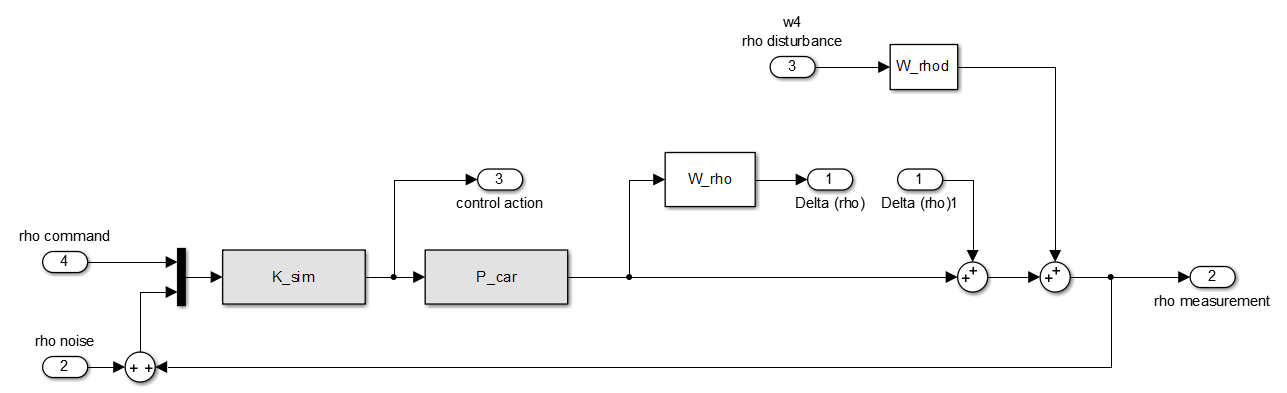
\includegraphics[width=.47\textwidth]{pics/model_car_unweighted.png} 
  \caption{Unweighted plant}  
  \label{figure:model_car_unweighted}
\end{figure}


\begin{figure}[h]
\centering
  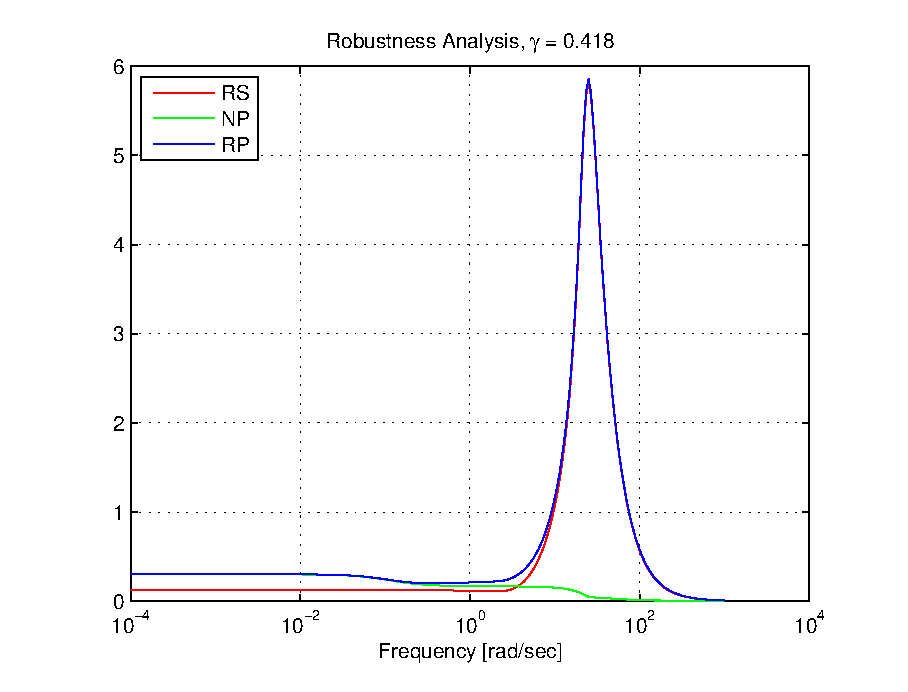
\includegraphics[width=.47\textwidth]{pics/RP_before_DK} 
  \caption{Robustness analysis of a $H_{\infty}$ controller}  
  \label{figure:RP_before_DK}
\end{figure}



\subsection{D-K iteration}

As a next step, a D-K iteration was performed. This had the result of an increased robustness, as Figure \ref{figure:RP_after_DK} shows. The values of the stability and performance analysis all have magnitude smaller than one, which means that stability is guaranteed while the performance requirements can be met.

\begin{figure}[h]
\centering
  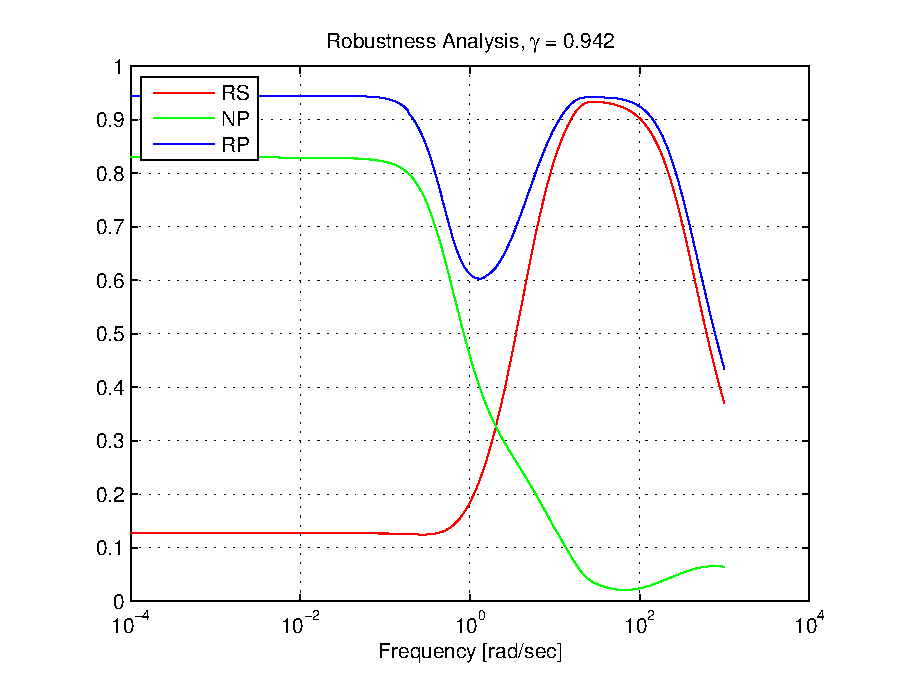
\includegraphics[width=.47\textwidth]{pics/RP_after_DK} 
  \caption{Robustness analysis after D-K iteration}  
  \label{figure:RP_after_DK}
\end{figure}

In order to compare the performance, a step response is shown in Figure \ref{figure:step_comp_02}. It can be seen that the system acts slower but with fewer oscillations. The poles of the closed loop system were found to be negative wherefore the system is stable.


\begin{figure}[h]
\centering
  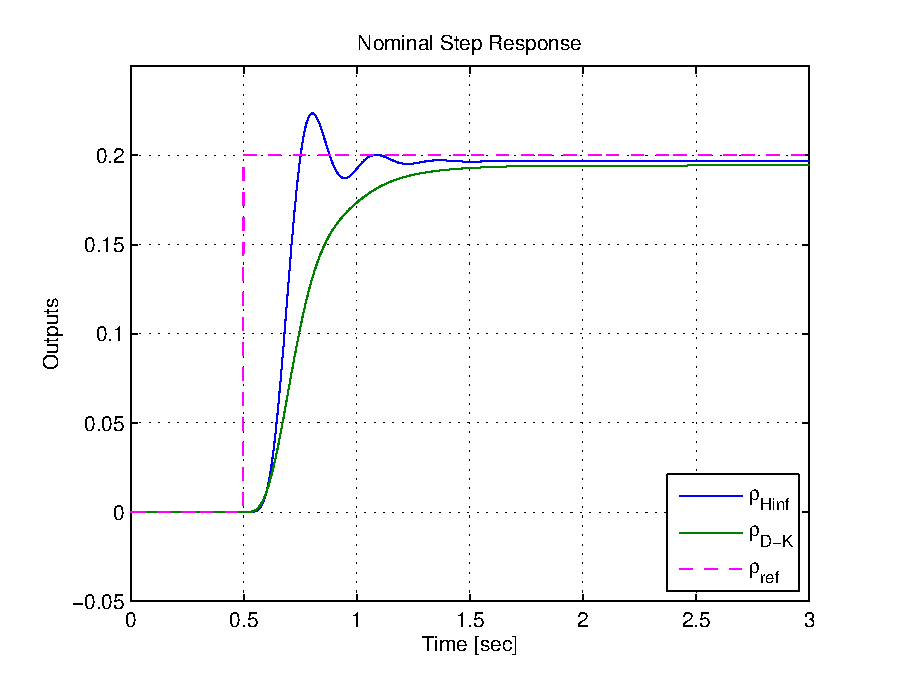
\includegraphics[width=.47\textwidth]{pics/step_comp_02} 
  \caption{Step response for different controllers}  
  \label{figure:step_comp_02}
\end{figure}


\section{Conclusions}

The simulation results have shown that the resulting controller is able to control a car on two wheels. Moreover, the robustness analysis showed that the performance requirements can be fulfilled as well as different perturbations representing modelling uncertainty can be handled.


\section{Future Work}

After the design of the presented controller, future work includes:

\begin{itemize}
\item Implementation of the controller on the real system
\item Changing the controller in order to control the position. This would also comprise the evaluation of a sensor which is suitable to track the vehicles position (e.g. GPS or optical flow)
\end{itemize}

 
 
 
\begin{thebibliography}{1}

\bibitem {bib:arndt} {\sc Arndt~D. et al.}: {\it Two-Wheel Self-Balancing of a Four-Wheeled Vehicle}. Article in IEEE Control Systems, 2011

\bibitem {bib:liu} {\sc Liu~K. et al.}: {\it Two-wheel self-balanced car based on Kalman filtering and PID algorithm}. Conference Paper, IEEE IE\&EM 2011


\end{thebibliography}


% that's all folks
\end{document}


